\chapter{Evaluation}
\label{chapter:evaluation}

In order to be worthwhile, skip regex must be faster than standard
regex and there must be ample opportunity to apply them. To evaluate
the degree to which skip regex meet these goals, we perform a number
of experiments. In section \ref{section:microbenchmarks}, we present a
series of micro benchmarks to demonstrate
the performance of skip regex under specific conditions. The micro
benchmarks show that the performance of skip regex is
at least as good as the equivalent standard regex execution, and 
is often significantly better.
In section \ref{section:logparsingcase} we perform a case study walking
through the steps a programmer might take while parsing logs from
an Apache Kafka instance.
In section \ref{section:applicability} we focus on the usefulness of
skip regex for regular expressions found in the wild. We scraped
\verb'crates.io', the Rust package repository,
for regular expressions and tested to see how applicable each of the 
optimizations we perform are. 

All benchmarks were run
on the same 5 year old Lenovo Y500 with a 4 core
Intel\textregistered Core\textsuperscript{TM} i7-3630QM CPU @
2.40GHz and 8 GiB of RAM.

\section{Micro Benchmarks}
\label{section:microbenchmarks}

Microbenchmarks alone are not typically enough to develop a high
level understanding of application performance, yet they remain
quite useful for demonstrating performance edge cases. Put another
way, microbenchmarks are excellent tools for performance story
telling. Sometimes such story telling can be used to deceive,
but we will attempt to avoid any deception and instead focus
on the performance trade-offs of skip regex.

The micro benchmarks we present in this section each consist of
a regex template and an input template which get instantiated
based off of some scaling factor and then run with different
backends. The scaling factor typically increases the input
size by a constant number of characters, and less commonly
increases the regex size. We indicate the parts of the
input multiplied by the scaling factor by raising them
to the \verb'n'the power. For example, \verb'abbbb' with \verb'a'
repeated according to the scaling factor is written as
${\tt a}^n{\tt bbbb}$. We run each microbenchmark at a
number of different scaling factors using Rust's built in
benchmarking facility, which takes a number of samples before
reporting the average runtime plus the spread between the minimum
and maximum runtime. We indicate the spread by attaching error bars to
each datapoint in our scatter plots.

In order to demonstrate the utility of different optimizations,
we execute the benchmarks with different engines and different
optimizations enabled. The standard regex engines are called
\texttt{baseline\allowbreak -\allowbreak backtrack} and
\texttt{baseline\allowbreak -\allowbreak pike}, while the
skip backends are called \texttt{skip\allowbreak -\allowbreak backtrack}
and \texttt{skip\allowbreak -\allowbreak pike},
with a number of optimization specifiers tacked onto the end to
indicate which optimizations have been enabled. For example,
\texttt{skip\allowbreak -\allowbreak backtrack\allowbreak -\allowbreak
        ds\allowbreak -\allowbreak es}
indicates that the skip backtracker with $.*$ scanning and $e*$ scanning
enabled. When all optimizations are enabled we shorten this to
\texttt{skip\allowbreak -\allowbreak backtracker\allowbreak -\allowbreak
all}.

Figure \ref{fig:8000:all} provides a comparison between all the
different benchmarks at a scaling factor of 8000.

\begin{figure}
\caption{Benchmarks at Scaling Factor 8000}
\label{fig:8000:all}

\makebox[\textwidth]{
    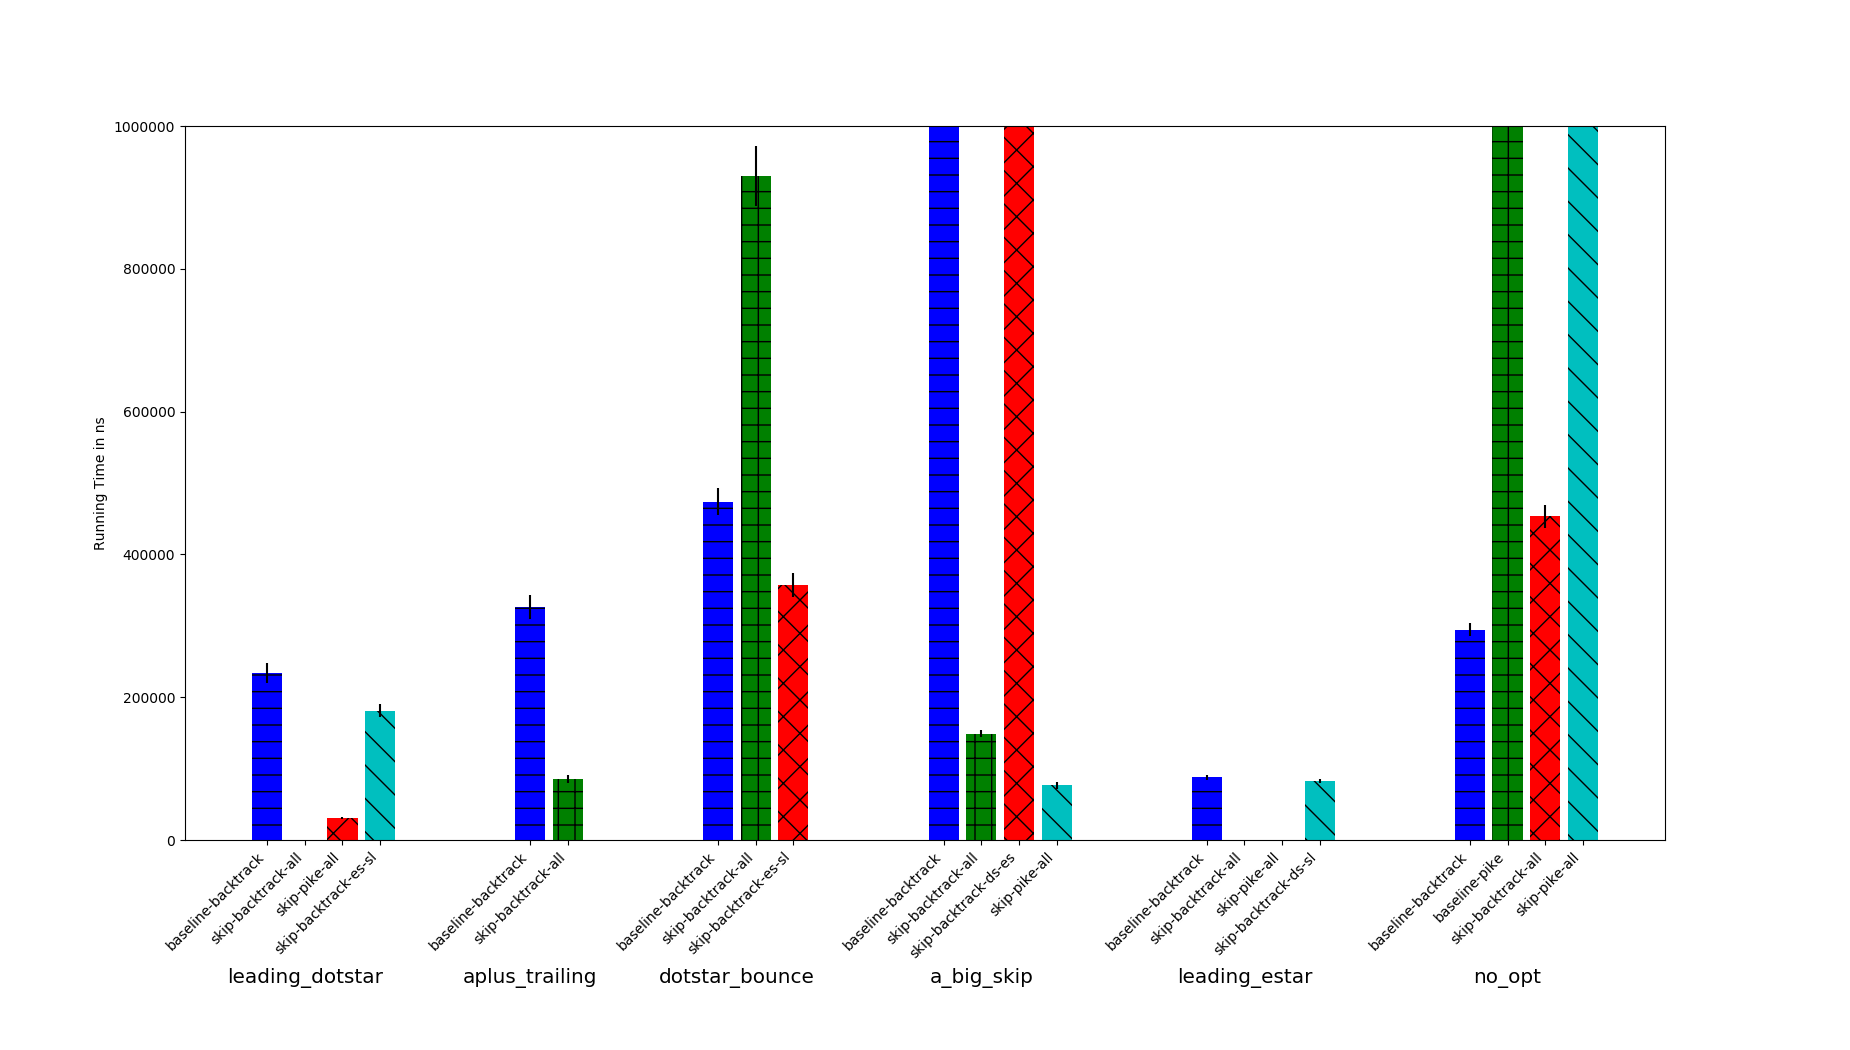
\includegraphics[width=\paperwidth]{resources/8000-bar.png}
}
\end{figure}

% TODO: open up a documentation PR so that other people don't
%       have to go digging through rustc source to figure out
%       what the +/- means.

\subsection{Best Possible Case: A Big Skip}

The best possible case for skip regex is where a regex is composed
entirely of large literals. In such a case a standard regex engine
must laboriously test every input character, while a skip regex
engine is allowed to traverse the input in a few big hops. Figure
\ref{fig:a:big:skip} illustrates just such a case. Here we executed the
regex ${\tt /aaaa}^n{\tt (bbbb)}{\tt cccc}^n{\tt /}$ on
an input of the form ${\tt aaaa}^n{\tt bbbb}^n{\tt cccc}$.
As we might expect,
the graph shows that both the skip Pike VM and the skip backtracker
beat out the non-skip backtracker quite handily, with the running time
of the skip engines remaining virtually flat as the running
time of the standard backtracker grows linearly with the scaling factor.
The performance improvement is entirely due to the literal skip
optimization, as shown by the fact that the performance of the skip
backtracker with literal skipping disabled is closer to the performance
of the \verb'baseline-backtrack' configuration.

\begin{figure}
\caption{A Big Skip}
\label{fig:a:big:skip}

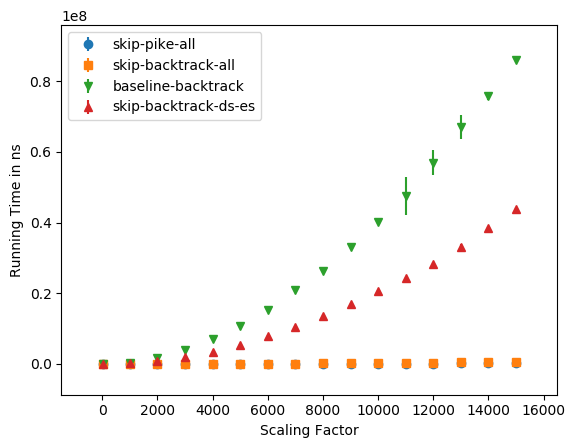
\includegraphics{resources/a-big-skip.png}
\end{figure}

\subsection{Leading $.*$}

While not quite as good as being able to traverse the whole input
in a few hops, a leading $.*$ which never needs to rely on non-determinism
A standard regex must go through the expensive process of spawning
two new threads for each character of input, one of which will die after
each step. By contrast, a skip regex engine can drop right into a fast substring
search algorithm. We produced figure \ref{fig:leading:dotstar} by executing
\verb'/.*(aaaa)/' on ${\tt b}^n{\tt aaaa}$.
The graph shows that all the engines are linear
in the size of the input, but the constant factor for the skip engines
is so much lower that they appear nearly constant time.

\begin{figure}
\caption{Leading $.*$}
\label{fig:leading:dotstar}

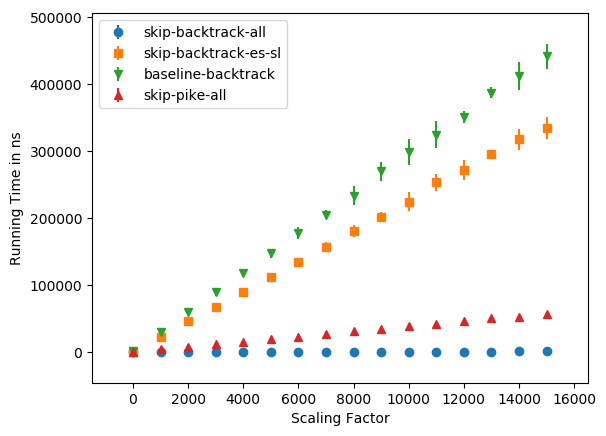
\includegraphics{resources/leading-dotstar.png}
\end{figure}

\subsection{$.*$ Bounce}

It would not be fair to showcase the best possible case for the
$.*$ scan optimization without also demonstrating the worst
case. If the literal terminator appears many times before the
end of the repetition, the skip engine will be forced to
rapidly enter and leave the substring search algorithm, spawning
two new threads on every iteration. Such an execution profile
is no better than a standard regex execution.
To demonstrate this worst case situation we executed
the regex \verb'/.*a(bbbb)/' on ${\tt ca}^n{\tt bbbb}$. Note
that it is \verb'ca' that is repeated according to the scaling factor,
not just \verb'a'. Figure \ref{fig:dotstar:bounce}
shows that the skip backtracker is slower than the standard
backtracker due to the overhead of switching back and forth between the
literal searcher and main engine loop. When the $.*$ optimization is
turned off, the skip backtracker behaves just like the standard
backtracker. This example was constructed to showcase the worst
case for the $.*$ scan optimization, but it seems less likely to appear
in the wild than the best case.

\begin{figure}
\caption{$.*$ Bounce}
\label{fig:dotstar:bounce}

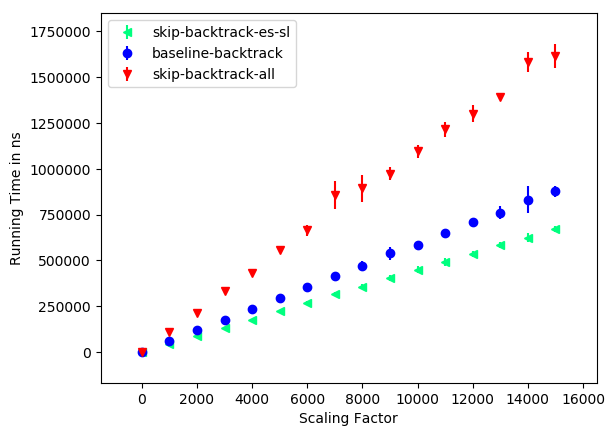
\includegraphics{resources/dotstar-bounce.png}
\end{figure}

\subsection{Leading $el$ Scan}

The $el$ scan optimization only really has a best case, because
the scan is always guaranteed to find the literal terminator. The
effectiveness of the optimization is entirely determined by the
size of the input, something which can be completely described
by one experiment. We produced figure \ref{fig:leading:noncontaining:estar}
by executing the regex \verb'a*foo(bar)' on ${\tt a}^n{\tt foobar}'$.
Note that fact that \verb'foo' cannot appear in any of the strings
in the language of \verb'/a*/' is determined statically, so no
runtime cost is paid. Just as in the ``Leading $.*$'' experiment,
all engines are linear, but the skip backends are so much faster that
they appear almost constant time.

% TODO: compile time.

\begin{figure}
\caption{Leading $el$ Scan}
\label{fig:leading:noncontaining:estar}

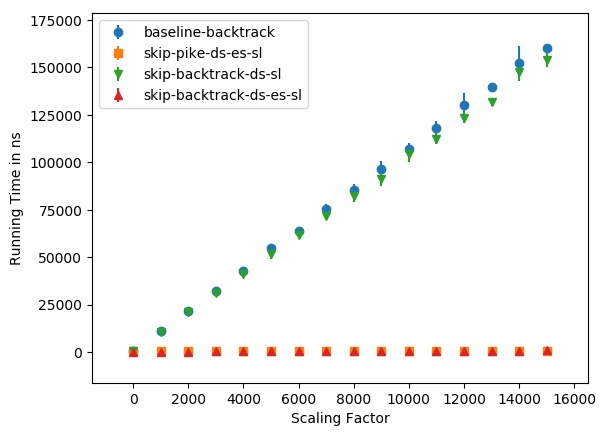
\includegraphics{resources/leading-noncontaining-estar.png}
\end{figure}

\subsection{Trailing $.*$}

When an expression contains a trailing $.*$ it can be compiled
directly to a \verb'goto-end' instruction. To showcase the
performance impact of this optimization we executed the
regex \verb'(a+).*' on ${\tt a}^n{\tt b}^n$
Figure \ref{fig:aplus:trailing} shows the results. Both the standard
and skip engines have to process the first half of the input
by spawning new threads, but the skip engine is always able
to skip the second half. This results in a noticeable speedup.

\begin{figure}
\caption{Trailing $.*$}
\label{fig:aplus:trailing}

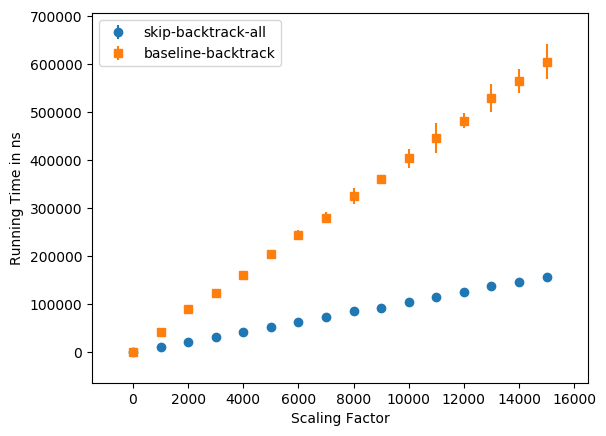
\includegraphics{resources/aplus-trailing.png}
\end{figure}

\subsection{No Opt}

In some cases no optimizations can be usefully applied to a skip
regex. We include such a case to demonstrate that with the exception
of a bouncing $.*$ optimization, the performance of skip regex is
no worse than that of standard regex. We produced figure 
\ref{fig:justtwo:branch}
by executing the regex \verb'/(ab|ac)*/' on ${\tt ab}^n$ with
the while input multiplied by the scaling factor. The fact that the
two branches of the alternative have intersecting first sets
(in particular $\{a\}$ and $\{a\}$), means that skip optimizations
can't be applied, and there is no clever way to get out of
executing the full kleene star. There is still some spread between
the different engines, most notably between the Pike VMs and the
bactrackers, as backtrackers are generally faster. The skip Pike VM
has a higher constant factor than the standard Pike VM when optimizations
are not helping out because of the increased complexity of its runnable
thread queue. There is a slight difference in constant factor between
the skip backtracker and the standard backtracker, but it is negligible.

\begin{figure}
\caption{No Opt}
\label{fig:justtwo:branch}

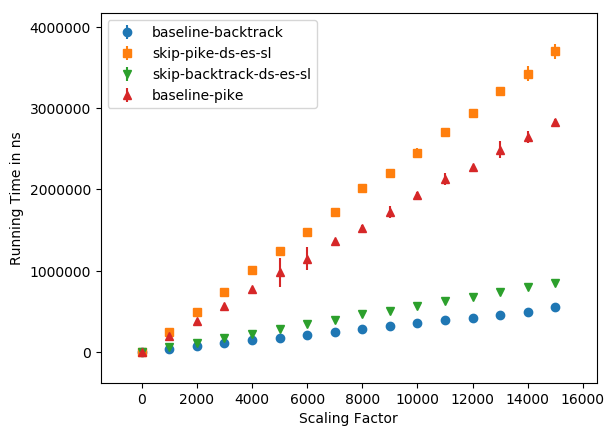
\includegraphics{resources/justtwo-branch.png}
\end{figure}

\section{Log Parsing: A Case Study}
\label{section:logparsingcase}

Regular expressions can be used in core application code, but they
are quite frequently used in a more improvisational capacity.
Searching through source code in an editor, filtering and parsing
the output of a previous command in a unix pipeline, or aiding
the construction of quick one-off scripts are all examples of
common use cases for regular expressions. We present an example
walking through the use of skip regex in pre-validated mode
to scrape an Apache Kafka debug log file. This case study
demonstrates the utility of skip regex beyond the library context
illuminated by the \verb'crates.io' figures presented in section
\ref{section:applicability}.

We present this case study as a partial literate program,
including just the most interesting kernel from the actual
program that we wrote. The full code for our scraping program
and the scripts used to generate test data can be found at
\cite{PailesSkipRegexCaseStudy}.

\subsection{Experimental Setup}

Apache Kafka is a Java-based distributed queuing system with
named event categories called topics consisting of several
queues called partitions. Like many network applications,
Kafka contains extensive and configurable debug logging,
which makes it a good source of test data. We configured
Kafka to log as promiscuously as possible and used a simple
python script to repeatedly publish and consume from a 
\verb'test' topic. We used the resultant log file as input
to our scraping script. To make the input log large enough
to observe a difference in performance measured in tenths of
a second, we concatenated the log to itself several times.

To collect and plot results we ran each benchmark 100
times, and used the unix \verb'time' tool to extract
the amount of user time that the program spent on each
run. We present the results in a series of box and whisker
diagrams. The boxes indicate the upper and lower quartiles
of the data.

\subsection{Summarizing Append Events}

When a new message is appended to a Kafka queue it notes some
metadata about the message such as its size and the offset to
which it was written in the partition. An example of such a log
line can be found in figure \ref{fig:appendevent}. To extract
the offset and number of bytes written from such lines we
used a regex defined as

\begin{verbatim}
let append_line = r"^.* with first offset: ([0-9]+).*value=([0-9]+).*$";
let append_re = regex!(append_line, args.flag_validate);
\end{verbatim}

\noindent
The \verb'append_line' variable contains Rust raw string containing the regex we
plan to use, and \verb'append_re' is a compiled regex object ready for
execution. \verb'regex!' is a previously defined Rust macro which
constructs a regex from its first argument, using the standard engine
if the second argument is false and a skip based engine in validation
mode if the second argument is true. Our program accepts a command
line flag indicating which sort of backend it should use in order
to facilitate comparison.

Once we have constructed our regex we can iterate over our input
file and extract statistics from each line.

\begin{verbatim}
let file = File::open(&args.arg_log_file).expect("cannot open log file");
let file = BufReader::new(file);
for line in file.lines().filter_map(|result| result.ok()) {
    stats.no_lines += 1;
    if args.flag_append {
        scrape_append(&append_re, line.as_bytes(), &mut stats);
    }
} 
\end{verbatim}

The first few lines are just a standard Rust song and dance to
iterate over the lines of a file, buffering the input and filtering
out any errors. We guard scrapping append data with a flag to allow
us to study its performance in isolation or along with other
scraping tasks. The \verb'stats' variable is a struct containing the summary
statistics we have collected so far about the log file. By far
the most interesting thing going on in this block of code is
the fact that \verb'scrape_append' has no way of knowing which
sort of regex engine is using. When used in validation mode,
skip regex can be used for all the same things that standard
regex can be used for.

The \verb'scrape_append' function keeps track of the min and max log
indices we have seen appended to so far, the total
number of bytes written, and the total number of appends.
It is defined as

\begin{verbatim}
fn scrape_append<'a>(re: &Regex, line: &'a [u8], stats: &mut Stats) {
    match re.captures(line) {
        Some(caps) => {
            stats.appends += 1;
            let off = String::from_utf8_lossy(&caps[1])
                            .parse::<usize>().unwrap();
            stats.max_append_offset =
                cmp::max(stats.max_append_offset, off);
            stats.min_append_offset =
                cmp::min(stats.min_append_offset, off);

            let nbytes = String::from_utf8_lossy(&caps[2])
                            .parse::<usize>().unwrap();
            stats.total_bytes_written += nbytes;
        }
        None => (),
    }
}
\end{verbatim}

It asks for the capture groups of the regex,
then updates all the relevant statistics if a match occurs.

\begin{figure}
\caption{Example Append Event Log Line}
\label{fig:appendevent}

\texttt{[2018-02-15 11:39:30,073] \allowbreak TRACE Appended \allowbreak
message set \allowbreak to log \allowbreak test-0 with \allowbreak
first offset: \allowbreak 1000, next offset: \allowbreak 1001, and
messages: [(record=\allowbreak DefaultRecord(\allowbreak
offset=1000, \allowbreak timestamp=-1, \allowbreak key=0 bytes,
 value=14 \allowbreak bytes))] \allowbreak(kafka.log.Log)
}
\end{figure}

\paragraph{Results}

Running our scraping script on a 25M log file showed a
respectable speedup for skip regex (figure \ref{fig:append}).
Our script reported that only 3.51\% of lines matched, so
most of the time was spent in the DFA discarding non-matching
lines in both cases. The 26.03\% difference in user
time then comes from the 3900 matching lines. We stripped
away the non-matching lines with grep to more directly observe
the difference in performance of the two NFA simulations we got
the shown in figure \ref{fig:append:just:match}.
When the NFAs must be used every time the difference in performance
is even more pronounced, demonstrating that the difference in performance
must be in the NFA simulation. The NFA simulation is the slowest part of
the system, so Amdahl's Law tells us that improvements to it ought to have
a disproportionately positive impact on overall runtime (\cite{Amdahl1967}).
This example confirms that intuition by showing that even when only a small
subset of the input lines match, NFA performance really matters.

\begin{figure}
\caption{Parsing A 25M Kafka Log for Append Events.}
\label{fig:append}

The center line indicates average running time, the
box indicates the lower and upper quartiles, whiskers show
the range of values, and flier points show outliers.

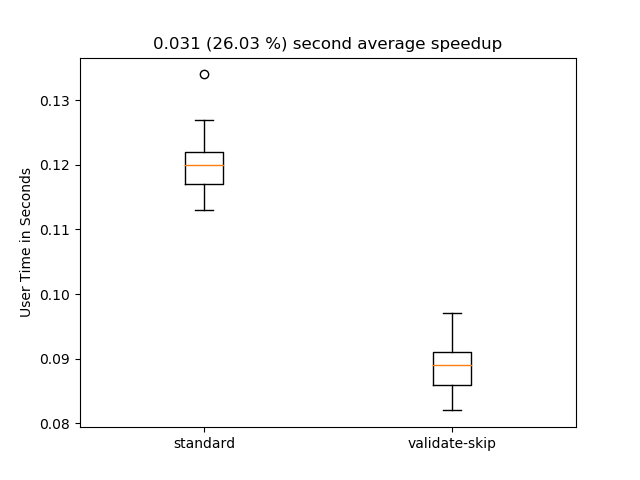
\includegraphics{resources/append.png}
\end{figure}

\begin{figure}
\caption{Parsing 848K of Append Events}
\label{fig:append:just:match}

The input for this benchmark was synthesized by taking
only the lines that matched from the original 25M log file.

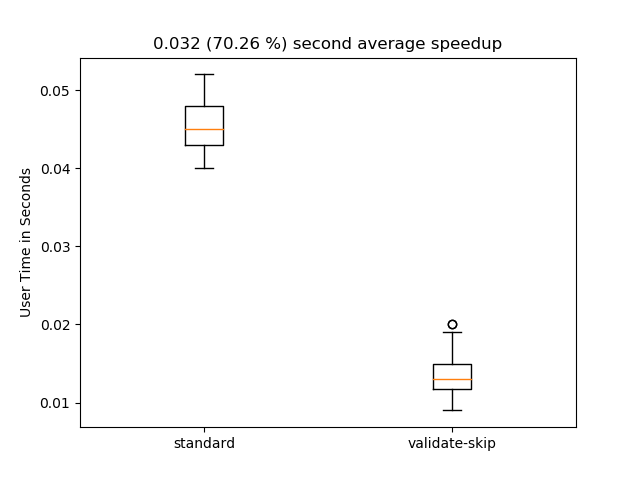
\includegraphics{resources/append-just-match.png}
\end{figure}

\subsection{Counting Scheduled Tasks}

Kafka has a number of scheduled tasks that can be used to track
the behavior of the server. Whenever one of these named
tasks happens, Kafka logs it with a line like the one
found in figure \ref{fig:namedevent}. We wanted to find out which
events were the most common, and how many in total there were.
To do so we needed to extract the event names using the
regex

\begin{verbatim}
let named_line = r".* scheduled task '(.+?)'.*";
let named_re = regex!(named_line, args.flag_validate);
\end{verbatim}

Declaration of \verb'named_re' follows the same pattern used above,
so we won't go over it again. To collect statistics about scheduled
tasks, we just added

\begin{verbatim}
if args.flag_named {
    scrape_named(&named_re, line.as_bytes(), &mut stats);
}
\end{verbatim}

\noindent
to the body of the loop shown above. The \verb'scrape_named'
function is defined as

\begin{verbatim}
fn scrape_named(re: &Regex, line: &[u8], stats: &mut Stats) {
    match re.captures(line) {
        Some(caps) => {
            stats.named_events += 1;
            *stats.named_hist
                .entry(String::from_utf8_lossy(&caps[1]).to_string())
                .or_insert(0) += 1;
        }
        None => (),
    }
}
\end{verbatim}

\noindent
just like \verb'scrape_append', \verb'scrape_named'
tracks the total number of matching lines. \verb'stats.named_hist'
is a \verb'HashMap' that we use to build a histogram tracking the
total number of times that each event has shown up. Once we have
processed all of the input we determine and report the 10 most common
events with

\begin{verbatim}
let mut hist = stats.named_hist.drain()
    .map(|(e, n)| (n, e)).collect::<Vec<_>>();
hist.sort_by(|lhs, rhs| rhs.cmp(lhs));
let v = hist.iter().take(10).collect::<Vec<_>>();
for &(ref n, ref e) in v.into_iter() {
    println!("event {} happened {} times.", e, n);
}
\end{verbatim}

\noindent
which is a bit more work than we had to do to summarize the append
events. It might seem like this extra work should make the impact
of regex performance matter less, but our results show that
skip regex are still able to make significant improvements.
It is interesting to note just how much time is actually spent
on parsing during simple data munging tasks such as this one.

\begin{figure}
\caption{A Named Event Log Line}
\label{fig:namedevent}

\texttt{[2018-02-15 \allowbreak 11:39:25,728] \allowbreak TRACE \allowbreak
Beginning execution \allowbreak of scheduled \allowbreak
task 'isr-expiration'\allowbreak . \allowbreak(kafka.utils.\allowbreak
KafkaScheduler)
}
\end{figure}

% TODO: tense agreement

\paragraph{Results}

Figure \ref{fig:named} shows a nearly 50\% speedup for skip regex.
At the megabyte scale, the difference between 2 and 1 tenth of
a second is not that noticeable, but when log files start running
into the gigabyte range, as can easily happen for long running
networked systems like Kafka, it is a serious quality of life
improvement.

Figure \ref{fig:append:named} shows how our scraping script
performed when we ran both set of analysis at once. Again,
skip regex provide solid an improvement.

\begin{figure}
\caption{Parsing A 25M Kafka Log for Scheduled Tasks}
\label{fig:named}

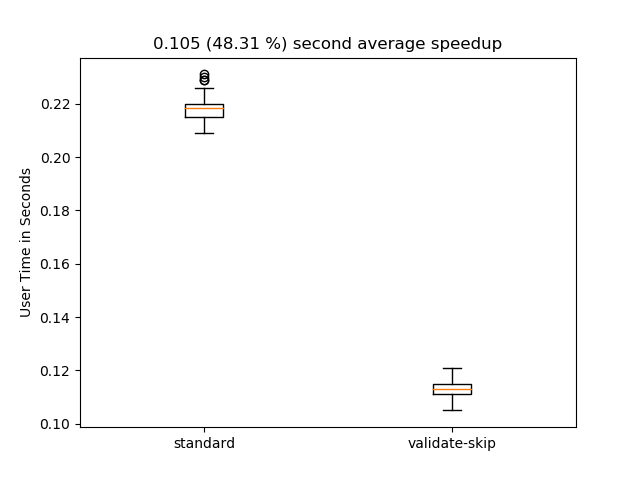
\includegraphics{resources/named.png}
\end{figure}

\begin{figure}
\caption{Parsing A 25M Kafka Log}
\label{fig:append:named}

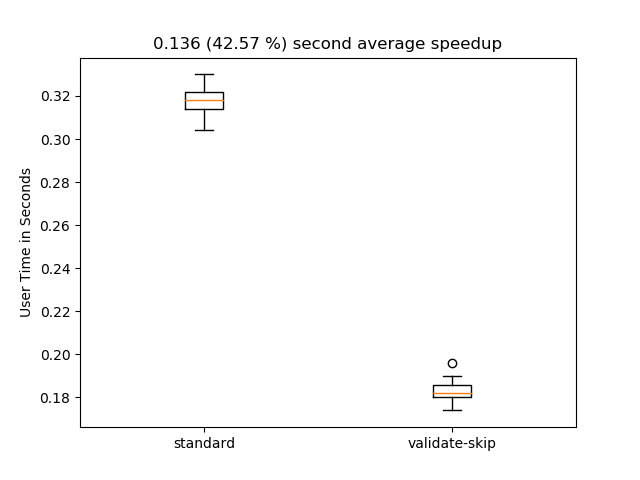
\includegraphics{resources/append-named.png}
\end{figure}

\section{Applicability}
\label{section:applicability}

It is hard to evaluate the applicability of the optimizations presented
in this thesis. It is quite easy to invent scenarios where each
optimization might be worthwhile, so any such examples \emph{alone} are
suspect. Existing regular expressions provide a better tool for
evaluating applicability, but it is important to watch out for
bias towards one particular application in any sample of existing
regex. It is also important to consider the fact that skip regex
can be used as more than just a faster regex engine. In situations
where a programmer might otherwise be inclined to directly encode
skips and scans to quickly parse some trusted input, they can
instead write skip regex with the intent of triggering optimizations.
Such optimization-aware usage cannot be evaluated by examining
existing regex.

A nice thing about extending an existing regex engine
with a decently sized user base is that a diverse group of developers
have written all sorts of different regex using the existing syntax.
To compile a list of such regex we pulled down all the
crates on \verb'crates.io' which depend on the regex crate, and
searched their source code for occurrences of the pattern
\verb'Regex::new\((r?".*")\)'. We only collected a subset of
the regex that could possibly be found, as there are ways to
produce a Rust regex without calling \verb'Regex::new', but
other methods of construction are unusual.

Once we had collected
a list of 487 regex, we ran them though our compiler, taking
note whenever an optimization was triggered. We found that
82.8\% of regex could have some sort of skip optimization
applied. Most of this number comes from the fact that 74.1\% of
regex could have a literal compiled to a skip,
by contrast only 6.5\% could have a $.*$ optimization applied and 8.6\% could
have a $e*$ optimization applied. When considering the skip
optimizations together we found that 15.0\% could have some sort of
scan optimization applied. It is heartening to see that most regex
can benefit from skip optimizations, though the relatively low number
of opportunities for scan optimizations is less so. While skip
optimizations have the greatest potential for speedup\footnote{By turning
a linear time operation into a constant time one.}, most skips
are relatively short.

It is worth taking these numbers with a grain of salt. \verb'crates.io'
is very library heavy, which likely biases the dataset towards
more complex and tricky regex. The more complex a regex gets,
the more opportunity for first set collisions there are, which gets
in the way of optimization. The sorts
of regex used to scrape log files or extract data in a unix pipeline
are more likely to have a linear feel than the regex found in
libraries. As an example, the regex we used in our
benchmark graphing scripts to parse the output
of \texttt{cargo \allowbreak bench}, Rust's benchmarking utility, was
\texttt{/test \allowbreak([a-zA-Z:\_]+) \allowbreak +... bench\allowbreak
      : \allowbreak+([0-9,]+) \allowbreak ns/iter \textbackslash
      (\textbackslash+/\textbackslash- \allowbreak
      ([0-9,]+)\textbackslash).*\$/},
which contains multiple different opportunities for skip optimizations,
but is not really general enough to put in a library. Contrast this
with the regex
\texttt{
/([0-9a-zA-Z]\allowbreak\{1\}\allowbreak/\allowbreak
[0-9a-zA-Z]\{1\}\allowbreak[:]\allowbreak\{1\})
\{5\}\allowbreak[0-9a-zA-Z]\allowbreak{1}\allowbreak[0-9a-zA-Z]
\allowbreak\{1\}/
}
found in the \verb'wifiscanner' crate, which does not allow for
optimization. It is possible for a one-off data munging script to include
such a complex regex, and for a library to include a simple one, but
it seems less likely. It is also worth noting the size of the corpus of
regex we collected; 487 is a large enough number to get 
percentages worth talking about, but it is not as large as it might
be for a more mature language ecosystem.

% TODO: discussion of skip regex time complexity
